\documentclass[10pt,a4paper]{article}
\usepackage[margin=18mm,top=16mm,bottom=16mm]{geometry}
\usepackage{fontspec}
\usepackage{xetexko}
\setmainfont{Helvetica Neue}[BoldFont={Helvetica Neue Bold},ItalicFont={Helvetica Neue Italic},BoldItalicFont={Helvetica Neue Bold Italic}]
\setmainhangulfont{Apple SD Gothic Neo}[BoldFont={Apple SD Gothic Neo Bold}]
\usepackage{graphicx}
\usepackage{xcolor}
\usepackage{enumitem}
\usepackage{titlesec}
\usepackage{caption}
\usepackage{wrapfig}
\definecolor{accent}{HTML}{2F5597}
\setlist{nosep,leftmargin=1.1em,topsep=2pt,itemsep=2pt}
\titleformat{\section}{\normalsize\bfseries\color{accent}}{}{0em}{}
\titlespacing*{\section}{0pt}{8pt}{3pt}
\captionsetup{font=small,labelformat=empty,skip=2pt}
\setlength{\parindent}{0pt}
\setlength{\parskip}{4pt}
\linespread{1.15}
\pagestyle{empty}

\begin{document}

{\Large\bfseries 줄어드는 영역 속 생존 경쟁을 대규모 게임 기록으로 분석하는 연구\par}
\vspace{3pt}
{\normalsize 배틀로얄 게임의 단계별 탈락 위험 분석 · 진행 중인 연구 소개 (2026년 10월)\par}
\vspace{3pt}
{\color{accent}\rule{\linewidth}{0.8pt}}

\section{무엇을 연구하고 있는가}
여러 행위자가 시간에 따라 줄어드는 영역 안에서 경쟁할 때, 누가 언제 탈락하는지를 대규모 이동·사건 기록으로 분석하고 예측하는 연구를 하고 있습니다.
관측 환경으로는 배틀로얄 게임 PUBG를 사용합니다.
이 게임에서는 최대 100명의 플레이어가 팀을 이루어 한 맵에서 경쟁합니다.
안전구역은 정해진 단계에 따라 줄어들고, 구역 밖에 있는 팀은 계속 피해를 입습니다.
게임사가 공개하는 경기 기록에는 모든 플레이어의 위치(약 10초 간격)와 교전, 아이템, 구역 변화가 시각과 함께 담겨 있습니다.
그래서 줄어드는 영역 아래의 생존을 대규모로, 같은 규칙에서 반복해서 관찰할 수 있습니다.

\section{핵심 질문}
한 단계가 끝나는 시점에 살아 있는 팀이 다음 단계 안에 탈락할 확률은 얼마이며, 그 위험을 무엇이 좌우하는지를 묻고 있습니다.
이 확률은 쓰임새가 분명합니다. 코치와 분석가는 경기를 복기할 때, 중계진은 주목할 팀을 고를 때, 개발사는 구역 설정을 조정할 때 이 값을 쓸 수 있습니다.
팀의 상태를 표현할 때는 서식지가 줄어들 때 생물 집단이 사라질 위험을 다루는 생태학의 관점을 빌렸습니다.
팀의 상태는 네 가지로 나타냅니다. 구역 경계에 얼마나 노출되어 있는지, 다음 구역까지 얼마나 이동해야 하는지, 주변에 경쟁 팀이 얼마나 많은지, 팀원이 몇 명 남았는지입니다.

\section{지금까지 한 일}
\begin{itemize}
  \item \textbf{데이터.} 공개 경기 13,948경기를 사용했습니다. 경기는 맵, 시점, 팀 규모에 따라 12개 유형으로 나뉩니다. 약 3억 2천만 건의 기록에서 약 82만 개의 `팀--단계' 예측 사례를 만들었습니다.
  \item \textbf{미래 정보가 섞이지 않는 예측.} 예측 시점보다 10초 이전의 기록만 입력이 되도록 처리 과정을 설계했습니다. 이후 기록을 모두 지워도 입력이 똑같이 만들어지는지 자동으로 검증했습니다.
  \item \textbf{공정한 비교와 원인 분해.} 가까운 선행 연구 두 가지를 같은 데이터와 같은 평가 조건에 맞추어 재구현했습니다. 하나는 단계별 활동 지표로 개인의 생존을 예측한 연구(Sagong 등, 2025)이고, 다른 하나는 게임사 KRAFTON이 공개한 실시간 우승확률 모델입니다. 이어서 입력 정보, 학습 목표, 모델 구조를 한 번에 하나씩 바꾸며 성능 차이가 어디서 오는지 분해했습니다.
\end{itemize}

\section{알게 된 것}
\begin{wrapfigure}{r}{0.43\linewidth}
\vspace{-12pt}
\centering
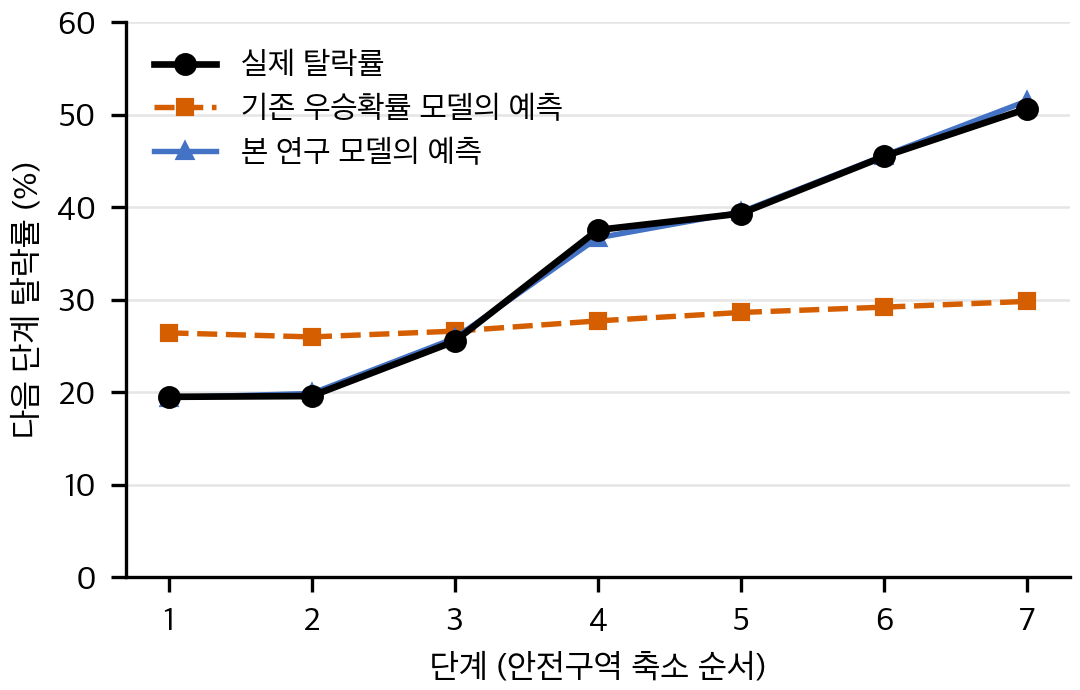
\includegraphics[width=\linewidth]{intro_calibration_ko.png}
\caption{단계가 진행될수록 실제 탈락률은 약 20\%에서 50\%로 오릅니다. 우승 순서를 학습하는 기존 모델은 이 변화를 거의 반영하지 못합니다.}
\vspace{-10pt}
\end{wrapfigure}
\textbf{위험을 좌우하는 요인.} 주변에 경쟁 팀이 많을수록, 다음 구역까지 이동 부담이 클수록 탈락 위험이 높습니다. 남은 팀원이 많을수록 위험은 낮습니다.
이 방향은 12개 경기 유형에서 대부분 일관됩니다.
구역 안쪽 깊숙이 있을 때의 보호 효과는 구역이 작아지는 중반 이후에 뚜렷해집니다.
이 네 요인만으로 150개 특징을 쓰는 모델 예측력의 약 80\%를 설명합니다.

\textbf{문제 정의가 성능을 좌우함.} 단계마다 달라지는 위험 수준을 직접 다루도록 문제를 정의한 모델이 기존 방법보다 잘 맞힙니다. 판별력(AUC)은 0.74에서 0.78로 올랐고, 12개 유형 모두에서 개선되었습니다.
성능 차이의 대부분은 모델 구조가 아니라 `무엇을 예측하도록 학습시키는가'에서 나왔고, 복잡한 신경망 구조가 더하는 이득은 작았습니다.
반대로 기존 모델의 원래 목적인 우승 팀 맞히기에서는 기존 모델이 더 잘 맞혔습니다. 각 방법이 자기가 겨냥한 질문에서 강하다는 점을 확인한 것입니다.

\section{현재 상황}
실험과 검증을 마쳤고, 결과를 IEEE BigComp 2027(빅데이터·스마트 컴퓨팅 국제학회) 논문으로 정리하고 있습니다. 투고 마감은 2026년 10월 16일입니다.
이 연구의 핵심 메시지는, 대규모 시공간 데이터에서 예측 대상을 정확히 정의하는 일이 모델 구조보다 성능 차이를 더 크게 좌우한다는 것입니다.

\end{document}
